\chapter{Materiali e Metodi}
Questo capitolo ha lo scopo di presentare il procedimento seguito per valutare l'ottimizzazione di una pipeline per l'analisi computazionale biofisica su nodi di cluster a basso consumo energetico.


In primo luogo sarà spiegato la componente principale creata per l'elaborazione, che implementa una parte del metodo GATK-LOD\ped{n}, e ne saranno approfonditi i singoli passaggi.

A seguire, saranno specificate quali computazioni sono state svolte, spiegando i motivi che hanno spinto a considerare talune, e il tipo di operazioni statistiche effettuate per modellare il prodotto delle analisi.



\section{Struttura delle simulazioni}
Il procedimento seguito dal sistema è suddivisibile in tre fasi: installazione, esecuzione e configurazione.


La prima di queste, la fase di installazione, evidenzia quali sono i fattori che permettono all'esecuzione di avvenire senza problemi.


In seguito, con la fase di esecuzione, è chiarita la struttura fondamentale del procedimento, ovvero la parte relativa all'algoritmo di analisi genetica, ed è definita la successione dei diversi passaggi: dalle estrazioni dei subset di DNA, fino alla produzione e semplicazione dei dati generati dal metodo.


Infine, sono esposte, nella fase di configurazione, le modalità di impostazione del programma, così da garantire una corretta gestione dei parametri e delle istruzioni da trasmettere ad esso.


\subsection{Installazione}
Il passaggio iniziale consiste nel predisporre l'ambiente di lavoro soddisfacendo i requisiti indispensabili per una valida esecuzione.

Nella preparazione di questa tesi, è stato scritto uno script apposito per questa fase preliminare, denominato \textit{installer.sh}, in modo da rendere questo procedimento compatto e più rapido.
Infatti, aver a disposizione un unico file da eseguire consente di automatizzare l'installazione e di garantire una gestione semplificato nel caso si parallelizzasse l'esecuzione su diversi nodi.

Questo eseguibile, in più, può risultare utile per coloro che sono già in possesso dei requisiti ma che preferiscono evitare di mischiare diversi ambienti di lavoro.
Ciò perchè l'installer aggiunge al bash script \textit{.bashrc} il percorso della directory Miniconda prodotta nell'installazione, così da indurre l'utilizzo di quei tool, tra cui \textit{Conda} e \textit{Snakemake}, inclusi nella medesima cartella.


Le due prerogative più importanti coinvolgono l'installazione di \textit{Conda}, che è inevitabile per l'attivazione degli ambienti, e ovviamente quella di \textit{Snakemake} per l'avvio del programma.


In seguito, sono richieste alcune librerie per Python, Pandas \cite{pandas} e Matplotlib \cite{Matplotlib}, che sono necessarie per una fase di sintesi dei file di benchmark e per le analisi statistiche.
In più, pur non avendo uno spessore di primo piano, sono essenziali i tool PyYAML e psutil, che colmano alcune lacune dei contenuti principali installati.


Dopo aver superato tali punti, è fondamentale equipaggiarsi del genoma umano di riferimento e dei dati genetici che si desiderano sequenziare.


In relazione al progetto ivi presentato, il genoma umano di riferimento è stato ottenuto via web dal sito ufficiale del IGSR(International Genome Sample Resource); mentre il campione di DNA esaminato è stato scaricato dal database pubblico DDBJ(DNA Data Bank of Japan).


Conclusi gli interventi preparatori, può essere avviata l'esecuzione del procedimento senza dover curare altri aspetti.


\subsection{Esecuzione}
La fase esecutiva comprende una serie di processi che si possono raggruppare in tre macro sezioni ben definite.
La prima di esse descrive il processo di estrazione dei sottogruppi, o subset, di sequenze di DNA che si sceglie analizzare.
La seconda presenta la pipeline per l'analisi del genoma e dichiara quali sono i prodotti attesi.
La terza racchiude un'operazione di riordinamento e di semplificazione di tali ultimi prodotti per agevolare le successive indagini statistiche.



\subsubsection{Estrazione}
\label{subsubsec: ext}
Gli oggetti delle analisi sono i subset genetici che si sceglie di estrarre dall'intero genoma del soggetto e per questo è lecito accennare a come avviene l'estrazione.

Il genoma del soggetto è solitamente contenuto in un file in formato di testo \textit{fastq} che contiene le sequenze di nucleotidi rilevate durante le analisi in laboratorio.
In questo progetto però, la rilevazione non è singola ma duplice e quindi i dati del paziente sono suddivisi in due file fastq accoppiati.
Ogni singola lettura contenuta nel \textit{fastq} è descritta da quattro linee che rappresentano: la marcatura della sequenza, la sequenza, l'identificazione del punteggio di qualità e il punteggio di qualità.


Nel lavoro inerente a questa tesi, è stato scritto uno script in Python(\textit{split.py}) che svolge l'operazione di estrazione e per il quale è sufficiente trasmettere da linea di comando gli estremi della sezione che si vuole ricavare; come indicato di seguito.
\begin{lstlisting}[language=Python]
$ python split.py {inizio} {fine}
\end{lstlisting}
Grazie all'inserimento degli estremi, il programma calcola il numero di reads desiderate, seleziona le linee corrispondenti(il quadruplo del numero di letture) e le trascrive in un nuovo file fastq.

Ai fini dello studio finale, la disposizione di sottogruppi sia con diversi numero di sequenze che in diverse regioni consente di analizzare nei particolari le proprietà di scalabilità delle computazioni.

Siccome il numero di letture contenute è enorme, ed essendo che ad ognuna corrispondono quattro linee, la dimensione del file fastq è di conseguenza molto grande; per questo risulta funzionale dotarsi di un meccanismo per l'estrazione di sottogruppi.

La creazione di un unico programma anche per l'estrazione dei subsets conferma l'impegno nel dotarsi di un sistema automatizzato che possa elaborare pressochè senza interventi esterni.


\subsubsection{Algoritmo di ricostruzione genetica}
Una volta creati i subsets, può essere applicata la pipeline di ricostruzione genetica, che è interamente contenuta nell'apposito Snakefile.
\'E importante notare che la procedura seguita è ripresa dal metodo GATK-LOD\ped{n} solamente in alcuni passaggi.
Tali passaggi, in particolare, sono concretizzati nello Snakefile da regole che si susseguono l'un l'altra in base alle dipendenze di ciascuna(sezione \ref{sec:SM}).

L'algoritmo GATK-LOD\ped{n} è stato integrato solo fino al riallineamento di GATK, escludendo quindi i passaggi di riallineamento Indel e di ricalibrazione dei punteggi di qualità.
Allo stesso tempo non sono state considerate le fasi fondamentali di chiamata alle varianti e l'implementazione del classificatore LOD\ped{n} di MuTect, vera novità del metodo GATK-LOD\ped{n}.

Questa forte selezione degli step è stata voluta appositamente per non appesantire lo studio sull'ottimizzazione computazionale e, quindi, è stato scelto di concentrare le analisi solo su quelle operazioni che formano le basi dell'algoritmo per l'indagine del DNA.
In tale maniera, è facilitata sia l'indagine sulla scalabilità che il confronto tra i diversi nodi adoperati, così da poter trarre rapidamente le prime conclusioni.

Le prime regole consistono nell'indicizzazione del genoma umano di riferimento per i software che partecipano al sequenziamento.
Queste coinvolgono il software di allineamento BWA, il tool di manipolazione Picard, il gestore di strumenti Samtools e i programmi affini a GATK.
Per le prime tre  applicazioni, questa operazione è portata avanti da una specifica opzione delle stesse, mentre per l'ultimo essa è inclusa già nell'uso di Samtools.

Terminate le indicizzazioni, è sfruttato BWA MEM per la mappatura del DNA del soggetto sul genoma di riferimento che, inoltre, produce un file di etichetta, in formato \textit{SAM}, che è sottoposto ad un riordinamento da parte Picard con l'assistenza della modalità SortSam.

Dopo essersi procurati i file \verb!sorted_bam!, è eseguito il comando MarkDuplicates di Picard per identificare le letture doppie ed è generato un nuovo file \verb!dedup_bam!.
Elaborando quest'ultimo, la regola successiva crea un indice(in un file \textit{bai}) per il file \textit{bam} in modo da velocizzare l'analisi dei dati nel \textit{bam}; ciò è realizzato da un'altra funzionalità di Picard chiamata BuildBamIndex.

Per concludere, supportati dalla direttiva RealignerTargetCreator, propria del pacchetto GATK, il contenuto del file \textit{bam} è riallineato localmente in modo da diminuire ed evidenzire il numero di variazioni presenti.

Per riassumere l'intero processo è possibile osservare la raffigurazione seguente \ref{fig:w}.
\begin{figure}[H]
\centering
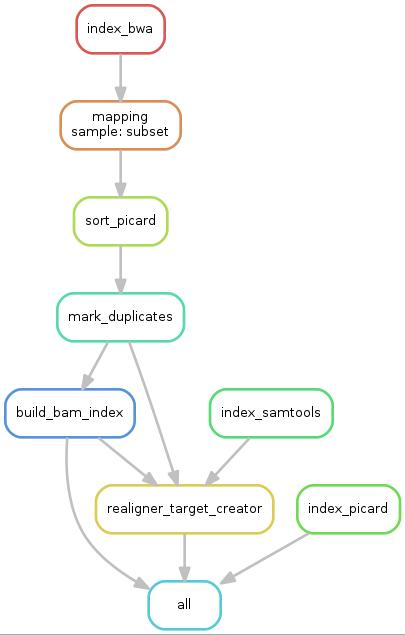
\includegraphics[scale=0.5]{Workflow.jpg}
\caption{Schematizzazione del procedimento implementato nella pipeline.}
\label{fig:w}
\end{figure}




\subsubsection{Organizzazione dei prodotti}
Il materiale su cui sono condotte le analisi statistiche sono i particolari tecnici e tempistici di ognuna delle regole completate.
Tali dati sono procurati, come già spiegato nella sezione \ref{subsubsec: SMb}, dalla direttiva benchmark in ogni passaggio.
Ciò significa che al termine dell'algoritmo sono prodotti tanti singoli file di benchmarking quante regole sono state completate, contando pure il caso in cui esse venissero ripetute ricorsivamente.
Per controllare la quantità di file e agevolare il futuro studio statistico, è stato scritto uno script in Python, denominato \verb!script_benchmark!.


Ogni file benchmark è dotato di un nome con funzione di etichetta; in particolare, la forma è la seguente.
\begin{lstlisting}[basicstyle=\fontsize{9}{6}\selectfont,breaklines=true]
benchmark_{name}_subset_{sample}_n_sim_{n_sim}_cputype_{cpu_type}_thrs_{thrs}_ncpu{n_cpu}.txt
\end{lstlisting}
Gli attributi contenuti nel nome indicano ordinatamente: il nome della regola completata, il tipo di campione analizzato, il numero della simulazione, il tipo di cpu utilizzata e il numero di threads e di cpu adoperati.
Mentre i primi due sono ricavati in automatico, gli altri fanno riferimento al file di configurazione dello Snakefile, come sarà spiegato nel paragrafo seguente.

Il lavoro svolto dallo script consiste quindi nel leggere ognuno dei file benchmark generati, considerare le etichette delle simulazioni e trasferire i dati incolonnati in un'unica tabella.
La tabella risultante non è dotata, quindi, solo delle colonne predefinite da \textit{Snakemake} nell'operazione di benchmarking(\ref{subsubsec: SMb}), bensì è arricchita dai dettagli contenuti nell'etichettatura.
In particolare, i dati sono organizzati nella tabella in ordine crescente rispetto al numero di simulazione.

All'avvio di questo script è controllato se è presente una tabella con lo stesso nome: in caso affermativo, i nuovi dati sono accodati ai precedenti; al contrario, ne è inizializzata un'altra.
In particolare, è necessario accedere al codice sorgente dello script se si vuole modificare il nome della tabella.

Attraverso questo sistema, il prodotto finale della fase di esecuzione, ed un unico oggetto dell'analisi statistica, è una tabella che racchiude le proprietà relative alle simulazioni ultimate.


Prima di procedere con l'esposizione dello studio effettuato su tali tabelle, è indispensabile perfezionare la descrizione del procedimento, specificando le opzioni di configurazione su cui essa si struttura.


\subsection{Configurazione}
Le ultime componenti del procedimento da delineare sono le modalità che definiscono le condizioni sotto cui deve essere portata avanti la computazione.
Queste componenti sono riportate nei file di configurazione e, per questa tesi, sono stati scritti due file di questo tipo che corrispondono rispettivamente a \textit{Snakemake} e a \textit{Conda}.

Le informazioni necessarie allo Snakefile sono procurate dal file \textit{config.yaml}, il quale comunica a \textit{Snakemake} alcuni dettagli della simulazione e le indicazioni su certe dipendenze.


Gli attributi della simulazione completano semplicemente l'etichettatura dei file di benchmarking e, pur rivestendo uno ruolo marginale, tali etichette permettono allo script di organizzazione dei dati una lettura rapida e quindi un'istanza immediata della tabella.
Come già citato precedentemente, i dettagli trascritti nel file di configurazione sono il tipo di cpu sfruttata, il numero della simulazione, il numero di threads adoperati e il numero di cpu coinvolte.

\'E stato scelto di gestire queste informazioni come parametri per non irrigidire il programma, visto che le macchine e i meccanismi usati possono essere innumerevoli.
Nello specifico, per modificare questi dettagli nelle etichette è sufficiente agire da linea di comando, come indicato nel paragrafo 1.2.1.

Sempre nello stesso file di configurazione sono presenti alcune chiavi che rappresentato le dipendenze non implementabili automaticamente negli ambienti di \textit{Conda} per \textit{Snakemake}.
Innanzitutto, sono presenti due indicazioni necessarie per il meccanismo di mapping, che sono l'utilizzo di \textit{Illumina} come piattaforma e di \textit{WES-Nextera-Rapid-Capture} come libreria.
A seguire, è indicato l'indirizzo in cui si può trovare il Genome Analysis ToolKit, da applicare nella procedura di riallineamento.

Altre istruzioni sulla configurazione del procedimento sono richieste da \textit{Conda} per la creazione, attivazione e disattivazione degli ambienti di lavoro durante l'esecuzione di \textit{Snakemake}(paragrafo 1.2.1).

Sempre nell'ambito di questa tesi, è stato scritto solo un documento di configurazione relativo a \textit{Conda}, dato che la maggior parte dei processi necessita di un ambiente con le stesse caratteristiche.
Nello specifico, quest'unico file di riferimento è contenuto nella directory \textit{envs} ed è chiamato \verb!config_conda.yaml!.

I requisiti richiesti per l'ambiente sono soddisfatti istruendo espressamente \textit{Conda} all'utilizzo del canale \textit{bioconda} per procedere con l'installazione di tre software coinvolti nel sequenziamento: \textit{BWA}, \textit{Picard} e \textit{Samtools}.

Ora che la natura del sistema è stata argomentata e sono stati approfonditi pure le procedure configurative, è possibile illustrare il percorso di studio statistico effettuato, accompagnato da una presentazione del genere di simulazioni conseguite.

\section{Analisi statistiche}
Questa sezione si occupa di descrivere quale tipologia di studio statistico è stato compiuto e quali sono state le simulazioni sostenute. 
In particolare, saranno indicate quali caratteristiche sono state considerate e quali relazioni sono state oggetto di studio.     

L'analisi dei dati è stata condotta utilizzando il linguaggio di Python, sulla piattaforma iPython \cite{IPython}, e dotandosi delle librerie: Pandas, Matplotlib, Seaborn \cite{seaborn}, NumPy \cite{Numpy} e SciPy \cite{Scipy}.

Il trattamento dei dati ha coinvolto inizialmente le funzioni sui dataframe di Pandas per l'estrazione e la modifica delle tabelle finali ricavate al termine del procedimento.
Tali tabelle sono state ridotte ad un unico dataframe a cui sono state aggiunte quattro colonne per facilitare l'analisi. 
Le prime due contengono gli estremi del subset, ovvero la posizione della lettura iniziale e la posizione di quella finale, la terza contiene il numero di letture di ogni subset e la quarta il logaritmo del tempo di esecuzione.
Da questo unico contenitore sono state estratte progressivamente le tabelle utili alle varie analisi.

La sezione è divisa in tre sottosezioni, dove le prime due corrispondono alle caratteristiche principali su cui è stata condotta l'indagine statistica: il tempo di esecuzione e la memoria impiegata. 
L'ultima sezione include una semplice presentazione sul tipo di simulazioni che sono state completate.


\subsection{Analisi sul tempo di esecuzione}
\label{sbsec:Te}
Lo studio sul tempo di esecuzione è stato eseguito con lo scopo di delineare un andamento preciso di esso per ogni regola e per ognuna dei nodi adoperati.  

Inizialmente è stata derivata dal dataframe generale una tabella in cui ogni regola svolta corrispondesse a un subset e che quindi, non fossero presenti quelle regole indipendenti dal tipo di dati analizzati.
I lavori che dipendono dai dati sono, in ordine di esecuzione: la mappatura(mapping), l'ordinamento tramite picard(sort picard), la rilevazione dei duplicati(mark duplicates), la creazione dei file bam(build bam) e il riallineamento(realigner).
Al contrario, i processi indipendenti sono le indicizzazioni dello human reference per bwa, per picard e per samtools(index bwa, index picard e index samtools). 

In seguito è stata rappresentata su di un grafico la dipendenza del tempo di esecuzione di ogni regola rispetto alla grandezza del subset, identificando sullo questo stesso grafico un andamento per ogni nodo. 
In questa maniera è stato possibile verificare le differenze di prestazione tra le macchine server, adattando a ciascuna di esse una regressione lineare tra il tempo e il numero di sequenze del subset.

Una volta osservato l'andamento del tempo per ogni singola regola, l'attenzione è stata rivolta al tempo totale impiegato dalle regole dipendenti dal subset.
Per calcolare il tempo totale è stata creata una nuova tabella che contenesse tali regole, il tipo di cpu, il numero della simulazione e il tempo totale di esecuzione.

Un tale grafico consente di osservare come cresce il tempo di esecuzione complessivo all'aumentare del numero di letture e come ciò è influenzato dal tipo di macchina adoperata.

Terminato lo studio sulle regole dipendenti dalla grandezza dei subset, sono state brevemente considerate anche le regole indipendenti.
Anche in questo caso è stata tracciata su un grafico la dipendenza del tempo di esecuzione rispetto ad ogni regola, distinguendo il comportamento tra i differenti nodi.  

Infine, sono stati estratti subset di ugual grandezza ma con punti di partenza differenti, che hanno permesso di stimare la variabilità dei tempi di esecuzione in base alla posizione di partenza.

Il tempo impiegato per concludere ogni regola non è però l'unico fattore da prendere in considerazione, visto che per promuovere l'uso della parallelizzazione è indispensabile analizzare le modalità di utilizzo della memoria. 

\subsection{Analisi della memoria occupata}
\label{subsec:Mf}
La memoria fisica studiata è ottenuta grazie a Snakemake dal tool psutil sottoforma di una memoria detta RSS o \textit{Resident Set Size}(paragrafo \ref{subsubsec: SMb}). 

I dettagli sulla memoria che viene impiegata nei singoli processi è di fondamentale importanza per un corretto sviluppo di un futuro sistema parallelizzato.
Infatti, lo studio sull'andamento di tale memoria consente di verificare fino a che livello di scalabilità la cpu è proficua e quando il suo uso comincia a saturare.
Questi comportamenti indicano fino a che punto è possibile ottimizzare l'utilizzo dei core della cpu e identificano le memorie richieste dalle varie regole.
Distinguere quali sono i processi che necessitano maggiormente di memoria e quelli che ne utilizzano una scarsa percentuale, permette di conoscere quali sono i nodi per le varie regole che ottimizzano l'esecuzione.

Lo studio statistico condotto è stato interessato, come per le tempistiche, ad osservare il comportamento della memoria in base alle regole, ai subsets e ai diversi nodi.
Perciò, è stata inizialmente posta in relazione la memoria occupata da ogni regola con il numero di sequenze del subset, distinguendo le macchine.
Successivamente è stata eseguita la stessa operazione per le regole indipendenti dai dati ed infine, è stato studiato il comportamento della memoria lasciando invariato il numero di letture ma considerando diversi punti di partenza.
    

%\subsection{Analisi sui processi di input ed output} 
%Due ulteriori dati che Snakemake trascrive nel benchmark sono ottenuti da psutil, specificatamente dalla funzione \verb!disk_io_counters!, e sono il numero di bytes letti e quelli scritti dal processo.
%In particolare, questi sono rispettivamente nominati \verb!io_in! e \verb!io_out! e, come per la memoria rss, sono convertiti in megabytes da Snakemake. 
%
%Queste due proprietà garantiscono una conoscenza più approfondita di come la cpu partecipa alla computazione, evidenziando con quale intensità, espressa in MB, essa è coinvolta nelle distinte operazioni.
%Così come l'analisi di rss, la statistica sulle fasi di input ed output delinea gli effetti che i lavori causano sul nodo.
%Da queste informazioni si può trarre una valutazione su quanto al massimo è possibile servirsi della cpu e fino a che punto l'utilizzo di essa è efficace.
%
%Le analisi realizzate sono state le stesse che per la memoria rss e quindi sono stati studiati gli andamenti dell'input e dell'output per le regole dipendenti dai subset e pure quelle indipendenti.
%Ugualmente ai casi precedenti sono state valutate anche le dipendenze per il tipo di cpu e sono stati confrontati intervalli diversi aventi identico numero di letture.
%Non è stato presa in esame il valore complessivo per l'input e output nell'intero arco dell'esecuzione perchè da tale dato totale non è possibile ricavare alcuna informazione proficua.
 
\subsection{Le simulazioni completate} 
\label{subsec:simc}
Le simulazioni che sono state eseguite ai fini di questa tesi sono state scelte per valutare le performance sui nodi dei cluster a disposizione, in modo da evidenziarne la potenziale scalabilità.

I nodi low power adoperati, che sono stati illustrati nel paragrafo \ref{sec:LP}, sono stati impiegati in base alle loro diverse potenze computazionali e sono stati confrontati con un nodo del cluster bio8, utilizzato come riferimento per le macchine tradizionali.
È stato utilizzato un solo core per ognuno dei nodi in tutto l'arco del procedimento, rimandando ad un futuro sviluppo l'utilizzo di core multipli.  


Tutti i nodi hanno processato gli stessi subset di dati con un numero di letture iniziale pari a centomila fino a 3 milioni, passando per i multipli di centomila e di un milione.
In questo modo è stato possibile studiare le potenzialità delle macchine a processare dati identici con larghezza crescente e come questo incremento condiziona l'uso della cpu. 

Solamente sui nodi xeond e bio8 sono state portate avanti le simulazioni fino a subset con un numero di letture pari a 9 milioni, continuando da 3 milioni a scalare progressivamente di 1 milione.

Non sono stati fatti proseguire anche gli altri nodi perchè lo scopo della tesi è valutare il comportamento dei nodi su piccoli subset di dati e quali indicazioni questo possa dare per sviluppare un'esecuzione parallelizzata efficace.
Visto che per tale valutazione sono stati sufficienti i dati citati, solo le due macchine più performanti sono andati oltre per confermare le stime ottenute.

Ciò significa che tutte le simulazioni sono state svolte solamente su una piccola frazione delle letture in possesso. 
Infatti il numero di letture complessivo del paziente è 45 milioni e la massima grandezza di un subset condivisa tra tutti i dispositivi è stata di 3 milioni, che equivale circa al $6.7\%$.
Per xeond e bio8 invece, i subset sono stati allargati a 9 milioni, ovvero circa il $20\%$.
La tabella \ref{tab:sub_dim} mostra la dimensione occupata su disco dal numero di letture contenute nei subset. 

\begin{table}[H]
	\centering
	\begin{tabular}{lr}
		\toprule
			\text{numero di letture} & \text{dimensione su disco} \\
		\midrule
			\num{1e5}   & \text{2x 28.4\,MB} \\
			\num{1e6}     & \text{2x 284.9\,MB} \\
			\num{3e6}     & \text{2x 854.9\,MB} \\
			\num{9e6}     & \text{2x 2.6\,GB} \\
			\num{4.5e7}    & \text{2x 12.8\,GB} \\
		\bottomrule
	\end{tabular}
	\caption{Stima della dimensione dei subset in relazione al numero di letture. L'ultimo valore si riferisce all'intero paziente.}
	\label{tab:sub_dim}
\end{table}

Per ogni numero di letture la dimensione occupata su disco è il doppio perchè, come citato nel paragrafo \ref{subsubsec: ext}, sono generati in fase di estrazione due file \textit{.fastq} per ogni subset.

In dettaglio, queste simulazioni sono state ripetute dieci volte per i nodi xeond e bio8 mentre sono stata ripetute cinque volte per gli altri nodi.

Infine utilizzando lo script \verb!split.py! descritto nella sezione \ref{subsubsec: ext}, sono stati estratti subsets contenenti letture diverse, ma dello stesso numero, che sono stati studiati in una fase delle analisi.
L'unico numero di letture considerato è stato centomila e ciò è stato eseguito solo per i nodi dei cluster low power, e quindi non da bio8.

Nel capitolo seguente saranno esposti gli esiti più rilevanti, selezionati dai prodotti finali dell'analisi statistica effettuata sui dati delle simulazioni.  

